\documentclass{beamer}
\usepackage{beamerthemeshadow}

%\documentclass{article}
%\usepackage{beamerarticle}
%\usepackage{graphicx}

\usepackage{lastpage}

\usepackage{xcolor}
\usepackage{pgf}

\newcommand{\bi}{\begin{itemize}}
\newcommand{\ei}{\end{itemize}}
\newcommand{\be}{\begin{enumerate}}
\newcommand{\ee}{\end{enumerate}}
\newcommand{\bd}{\begin{description}}
\newcommand{\ed}{\end{description}}
\newcommand{\prbf}[1]{\textbf{#1}}
\newcommand{\prit}[1]{\textit{#1}}
\newcommand{\beq}{\begin{equation}}
\newcommand{\eeq}{\end{equation}}
\newcommand{\bdm}{\begin{displaymath}}
\newcommand{\edm}{\end{displaymath}}

\newcommand{\ft}[1]{
  \frametitle{\begin{tabular}{p{4in}r} \textcolor{white}{#1} & \small{\textcolor{white}{\thepage$~$ / \pageref{LastPage}}}\end{tabular}}
  \setbeamercovered{transparent=18}
}

\newcommand{\stepinv}{\setbeamercovered{invisible}}
\newcommand{\stopinv}{\setbeamercovered{transparent=18}}
\newcommand{\uncoverinv}[1]
{
  \setbeamercovered{invisible}
  \uncover<+->{#1}
  \setbeamercovered{transparent=18}
}
\newcommand{\ans}[1]{\textcolor{blue}{#1}}
\newcommand{\ansinv}[1]
{
  \setbeamercovered{invisible}
  \uncover<+->{\textcolor{blue}{#1}}
  \setbeamercovered{transparent=18}
}
\newcommand{\setinv}{\setbeamercovered{invisible}}
\newcommand{\setvis}{\setbeamercovered{transparent=18}}
\newcommand{\centerpic}[2]
{
  \begin{center}
  \includegraphics[#1]{#2}
  \end{center}
}
\newcommand{\h}[1]{\hat{#1}}
\newcommand{\ds}{\displaystyle}

\definecolor{mycolor}{rgb}{0.125,0.5,0.05}
\usecolortheme[named=mycolor]{structure}

\title[Empirical Significance of Learning with Firm-Specific Capital]{Empirical Significance of Learning in a New Keynesian Model with Firm-Specific Capital}
\author[Learning Week. St. Louis Federal Reserve Bank. July 2007.]{James Murray\\Indiana University}
\date{July 20, 2007}

\begin{document}

\frame{\titlepage}
\setcounter{page}{1}

\frame{
  \ft{Introduction}
  \bi
  \item Purpose: 
    \bi
    \item Estimate the empirical significance of learning.
    \item Determine what features of U.S. data constant gain least squares learning can explain.
    \ei
  \item Learning suggested to deliver features:
    \bi
    \item Inflation scares.
    \item Great moderation.
    \item Time varying volatility.
    \item Macroeconomic persistence.
    \ei
  \item Estimate a NK model with learning and RE by MLE.
    \bi
    \item Estimate with and without endogenous capital.
    \item Estimate under alternative initial conditions for beliefs of agents.
    \ei
  \item Examine forecast errors, evolution of shocks, and evolution of agents' coefficients.
  \ei
}

\frame
{
  \ft{Consumers}
  \textbf{Utility function:}
  \bdm U_0 = E_0^* \sum_{t=0}^{\infty} \beta^t \left[ \frac{1}{1-\sigma} \xi_t \left(c_t(i) - \eta c_{t-1}(i)\right)^{1-\sigma} - \frac{1}{1+\mu} n_t(i)^{1+\mu} \right] \edm
  \bi
  \item $E_t^*$: possibly non-rational expectations operator.
  \item $c_t(i)$: consumption at time $t$. 
  \item $n_t(i)$: labor supply at time $t$.
  \item $\xi_t$: common preference shock.
  \item $\beta$: discount factor.
  \item $\sigma \in (0,\infty)$: inverse of the intertemporal elasticity of substitution.
  \item $\eta \in [0,1)$: degree of habit formation.
  \item $\mu \in (0,\infty)$: inverse of the elasticity of labor supply.
  \ei
}

\frame
{
  \ft{Production}
  \textbf{Final good production:}
  \bdm y_t = \left[ \int_0^1 y_t(i)^{\frac{\theta-1}{\theta}} di \right]^{\frac{\theta}{\theta-1}} \edm
  \bi
  \item $y_t$ output of final good, $y_t(i)$ output of intermediate good $i$.
  \item $\theta \in (1,\infty)$: elasticity of substitution in production.
  \ei
  \textbf{Intermediate goods production:}
  \bdm \mbox{Model with capital:  } y_t(i) = z_t k_t(i)^{\alpha} \left(\nu^t n_t(i)\right)^{1-\alpha} \edm
  \bdm \mbox{Model without capital:  } y_t(i) = z_t n_t(i) \edm
  \bi
  \item $z_t$: common technology shock.
  \item $k_t(i)$: firm-specific capital good.
  \item $\nu$: gross growth rate of labor productivity.
  \ei
}

\frame
{
  \ft{Sticky prices}
  \bi
  \item Follow Calvo (1983) pricing: fraction $1-\omega$ firms re-optimize their price each period.
  \item Inflation indexation: Those who cannot re-optimize may adjust according to:
    \bdm \ln(p_{t}(i)) = \ln(p_{t-1}(i)) + \gamma \pi_{t-1} \edm
  \item With firm-specific capital (Woodford, 2005), leads to Phillips curve:
  \bdm \pi_t = \frac{\gamma}{1+\beta\gamma} \pi_{t-1} +  \frac{\beta}{1+\beta\gamma} E_t \pi_{t+1} + \kappa \h{s}_t \edm
  \item $\h{s}_t$: average marginal cost in the economy (percentage deviation from steady state).
  \item $\kappa$: function of many parameters.
  \ei
}

\frame
{
  \ft{Firm-Specific Investment}
  \bi
  \item Final good is converted to a firm-specific capital good.
  \item Investment of $I_t(i)$ leads to capital stock next period:
  \bdm k_{t+1}(i) = (1-\delta) k_t(i) + \mu_t I_t(i) - \frac{\phi}{2} \left[\frac{k_{t+1}(i)}{k_t(i)} - 1 \right]^2 k_t(i) \edm
  \bi
  \item $\mu_t$: common investment technology shock.
  \item $\delta$: depreciation rate.
  \item $\phi$: capital adjustment cost parameter.
  \ei
  \item Profit maximizing marginal cost:
    \bdm \h{s}_t = \frac{\mu+\alpha}{1-\alpha} \h{y}_t - \frac{\alpha(\mu+1)}{1-\alpha} \h{k}_t - \h{\lambda}_t - \frac{\mu+1}{1-\alpha} \h{z}_t, \edm
  \ei
}

\frame
{
  \ft{Market clearing}
  \bi
  \item Market clearing condition: 
    \bdm \mbox{Model with capital:  } y_t = c_t + I_t + g_t \edm
    \bdm \mbox{Model without capital:  } y_t = c_t \edm

  \item $g_t$: Exogenous demand shocks such as changes in government spending and net exports.
  \ei
}

\frame
{
  \ft{Monetary policy}
  \bi
  \item Model \textit{without} capital: interest rate responds to \textit{output gap}:
  \bdm \h{r}_t = \rho_r \h{r}_{t-1} + (1-\rho_r) \left(\psi_{\pi} \pi_t + \psi_y \tilde{y}_t \right) + \epsilon_{r,t} \edm
    \bi
    \item $\psi_{\pi} \in (0,\infty)$: feedback on inflation.
    \item $\psi_{y} \in (0,\infty)$: feedback on output.
    \item $\rho_r \in (0,1)$: smoothing parameter.
    \ei
  \item Model \textit{with} capital: interest rate responds to the deviation of output from steady state:
  \bdm \h{r}_t = \rho_r \h{r}_{t-1} + (1-\rho_r) \left(\psi_{\pi} \pi_t + \psi_y \h{y}_t \right) + \epsilon_{r,t} \edm
  \ei
}

\frame
{
  \ft{Exogenous shocks}
  \bi
  \item Non-policy shocks (percentage deviations from steady state) are AR(1):
    \bi
    \item Preference shock: $\h{\xi}_t = \rho_{\xi} \h{\xi}_{t-1} + \epsilon_{\xi,t}$ 
    \item Technology shock: $\h{z}_t = \rho_{z} \h{z}_{t-1} + \epsilon_{z,t}$ 
    \item Investment shock: $\h{\mu}_t = \rho_{\mu} \h{\mu}_{t-1} + \epsilon_{\mu,t}$ 
    \item Demand shock: $\h{g}_t = \rho_{g} \h{g}_{t-1} + \epsilon_{g,t}$ 
    \ei
  \item $\epsilon_{\xi,t}$, $\epsilon_{z,t}$, $\epsilon_{\mu,t}$, $\epsilon_{g,t}$, $\epsilon_{r,t}$ are independently normally distributed with mean zero.
  \ei
}

\frame
{
  \ft{Model without capital}
  \bi
  \item Re-write the model without capital in terms of the output gap.
  \item Notation:
    \bi
    \item Tilde denotes (percentage) deviation from fully flexible outcome.
    \item Superscript $f$ denotes fully flexible outcome.
    \item Superscript $*$ denotes steady state value.
    \ei

  \item Natural rate of interest:
    \bdm r_t^n = r_t^f - E_t \pi_{t+1}^f \edm
    \bdm r_t^n = \left(1-\rho_{r^n}\right) r^* + \rho_{n} r_{t-1}^{n} + \epsilon^{r^n}_{t}\edm
  \ei
}

\frame
{
  \ft{Model without capital}
  \bi
  \item Consumer first order conditions + market clearing:
    \bdm \tilde{\lambda}_{t} = E_t \tilde{\lambda}_{t+1} + \left(r_t - r_t^n - E_t \pi_{t+1}\right) \edm 
    \bdm \tilde{\lambda}_t = \frac{1}{ (1-\beta \eta)(1-\eta)}\left[ \beta \eta \sigma E_t \tilde{y}_{t+1} - \sigma(1+\beta \eta^2) \tilde{y}_t + \sigma \eta \tilde{y}_{t-1} \right] \edm

  \item Phillips curve:
    \bdm \pi_t = \beta E_t \pi_{t+1} + \kappa \left(\mu \tilde{y}_t - \tilde{\lambda}_t \right) + u_t \edm
    
  \item Cost push shock:
    \bdm u_t = \rho_u u_{t-1} + \epsilon^u_t \edm
  \ei
}

\frame
{
  \ft{General Form}
  \bi
  \item The New Keynesian model has the form:
  \bdm \Omega_{0} x_t = \Omega_{1} x_{t-1} + \Omega_{2} E_t x_{t+1} + \Psi z_t \edm
  \bdm z_t = A z_{t-1} + \epsilon_t \edm
    \bi
    \item $x_t$ vector of time $t$ variables, observable to agents at following time period.
    \item $z_t$: vector of time $t$ shocks, observable to agents in current period.
    \ei
  \item Rational expectations solution:
  \bdm x_{t} = G x_{t-1} + M z_{t} \edm
  \ei
}

\frame
{
  \ft{Learning}
  \bi
  \item Agents estimate elements of $G$ and $M$ by least squares.
  \item Agents know coefficients in $A$.
  \item $X_t$: vector of regressors: $X_t' = [1~ x_{t-2}'~ z_{t-1}']$.
  \item $Y_t$: vector of dependent variables: $Y_t = x_{t-1}$.
  \item $\hat{\phi}_t$: least squares estimate of the coefficients in $G$ and $M$.
  \item Information at available at time $t$: $x_{t-1}$, $z_t$. 
  \item Evolution of $\h{\phi}_t$ in recursive form:
    \bdm \hat{\phi}_t = \hat{\phi}_{t-1} + g R_t^{-1} X_{t-1} \left(Y_{t} - X_{t-1}' \hat{\phi}_{t-1}\right) \edm
    \bdm R_t = R_{t-1} + g (X_{t-1} X_{t-1}' - R_{t-1}) \edm
  \item where $g$ is the constant learning gain.
  \ei
}



\frame
{
  \ft{Estimation}
  \bi
  \item Method: Maximum likelihood estimation.
  \item Data: Quarterly data for 1960 through 2005.
  \item Model with no capital: 
    \bi
    \item CBO measure of the output gap.
    \item Annualized quarterly inflation rate of the GDP deflator.
    \item Annualized quarterly Federal funds rate.
    \ei
  \item Model with endogenous capital:
    \bi
    \item Real GDP per capita.
    \item Real private consumption per capita.
    \item Real gross private domestic investment per capita.
    \item Annualized quarterly inflation rate of the GDP deflator.
    \item Annualized quarterly Federal funds rate.
    \ei
  \item Calibrated parameters:
    \bi
    \item Model without capital: $\beta=0.99$, $\mu=0$ (perfectly elastic labor supply).
    \item Model with capital: $\beta = 0.99$, $\delta = 0.025$.
    \ei
  \ei
}

\frame
{
  \ft{Initial Conditions for Learning Algorithm}
  \bi
  \item $\hat{\phi}_t$ and $R_t$ must be initialized for estimation.
  \item MSV solution, expected outer product of the state vector under RE.
    \bi
    \item Much of learning theory valid for the neighborhood of the MSV solution.
    \item Initial conditions are supported by the micro-foundations.
    \item Problem: Learning dynamics smallest when near MSV solution.
    \ei
  \item Joint estimation:  
    \bi
    \item Problems: As many as 40 additional parameters (endogenous capital estimation).
    \item Motivation: illustrates how predictions depend on initial conditions.
    \ei
  \item Alternative approach: Use a VAR(1) from pre-sample data
    \bi
    \item Problem: latent variables are regressors - capital stock, structural shocks.
    \ei
  \ei
}

\frame
{
\ft{Results Without Capital Accumulation:\newline RE Solution for Initial Conditions}
\begin{scriptsize}
\hspace{-0.3in}
\begin{tabular}{|l|c|r@{.}l|r@{.}l|r@{.}l|r@{.}l|} \hline
Description & Parameter & \multicolumn{2}{|c|}{RE} & \multicolumn{2}{|c|}{Std. dev.} & \multicolumn{2}{|c|}{Learning} & \multicolumn{2}{|c|}{Std. dev.}  \\ \hline
Learning gain	&	$g$	&	&	&	&	&	0&0104	&	0&0048	\\
Habit formation	&	$\eta$	&	0&9953	&	0&0105	&	0&9470	&	0&0214	\\
Inverse elasticity sub.	&	$\sigma$	&	0&0830	&	0&0724	&	0&5057	&	0&4069	\\
Phillips curve slope	&	$\kappa$	&	0&0001	&	0&0001	&	0&0001	&	0&0001	\\
Price indexation	&	$\gamma$	&	0&9686	&	0&0458	&	0&9730	&	0&0172	\\
Interest rate smoothing	&	$\rho_r$	&	0&8449	&	0&0269	&	0&8943	&	0&0178	\\
Policy feedback on output	&	$\psi_y$	&	0&2073	&	0&0778	&	0&3346	&	0&0931	\\
Policy feedback on inflation	&	$\psi_{\pi}$	&	1&2812	&	0&2230	&	1&5895	&	0&3079	\\
Persistence nat. int. rate	&	$\rho_n$	&	0&9944	&	0&0081	&	0&9016	&	0&0273	\\
Persistence cost push	&	$\rho_u$	&	1&50E-6	&	0&0684	&	0&0000	&	0&0224	\\
Std. dev. nat. int. rate	&	$s_n$	&	0&0009	&	0&0005	&	0&1150	&	0&1065	\\
Std. dev. cost push	&	$s_u$	&	2&45E-6	&	3&40E-6	&	2&49E-6	&	3&00E-7	\\
Std. dev. policy shock	&	$s_r$	&	5&48E-6	&	3&40E-6	&	5&31E-6	&	3&30E-7	\\
Steady state inflation	&	$\pi^*$	&	7&9795	&	2&8442	&	5&6139	&	1&0109	\\ \hline
\end{tabular}
\end{scriptsize}
}

\frame
{
  \ft{Results Without Capital Accumulation:\newline RE Solution for Initial Conditions}
  \bi
  \item Learning gain statistically significantly different from zero.
  \item Habit formation and indexation remain significant sources of persistence.
  \item Learning model predicts lower steady state level inflation.
  \item Rest of the parameters are very similar.
  \ei
}

\frame
{
  \ft{Forecast Errors:\newline RE and Learning with RE initial conditions}
  \begin{center}
  \vspace*{-0.1in}\hspace*{-0.24in}\begin{tabular}{ccc}
  \multicolumn{3}{c}{\textbf{Rational Expectations}}  \\
  \small{Output gap} & \small{Inflation} & \small{Interest Rate} \\
  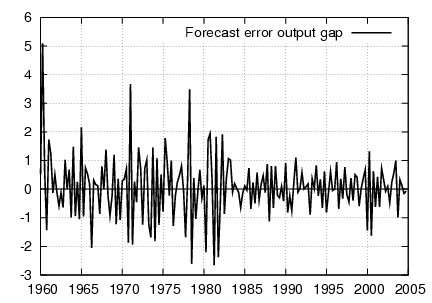
\includegraphics[scale=0.23]{plots2/re_Forecast_error_output_gap.png} & 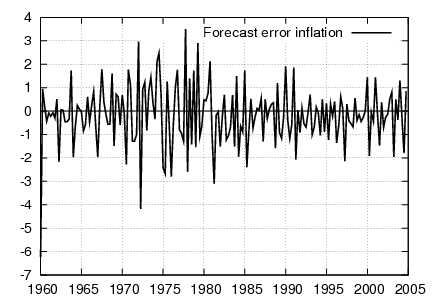
\includegraphics[scale=0.23]{plots2/re_Forecast_error_inflation.png} & 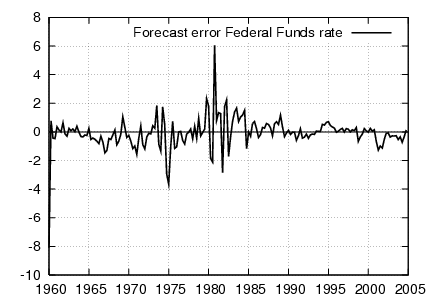
\includegraphics[scale=0.23]{plots2/re_Forecast_error_Federal_Funds_rate.png} \\ \\
  \multicolumn{3}{c}{\textbf{Learning (RE initial conditions)}}  \\
  \small{Output gap} & \small{Inflation} & \small{Interest Rate} \\
  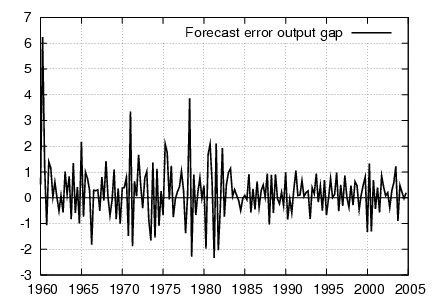
\includegraphics[scale=0.23]{plots2/initre_Forecast_error_output_gap.png} & 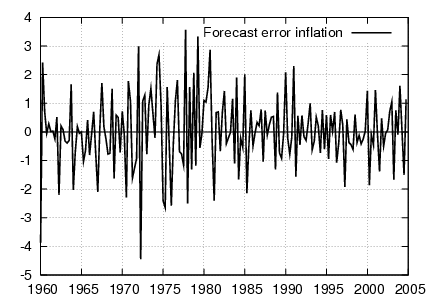
\includegraphics[scale=0.23]{plots2/initre_Forecast_error_inflation.png} & 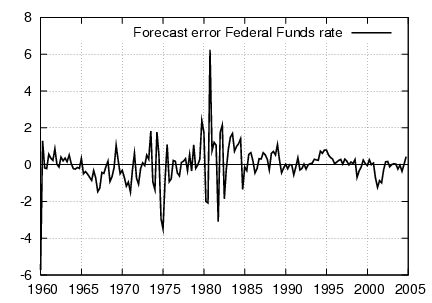
\includegraphics[scale=0.23]{plots2/initre_Forecast_error_Federal_Funds_rate.png} \\ \\
  \end{tabular}
  \end{center}
}

\frame
{
  \ft{Forecast Errors:\newline RE and Learning with RE initial conditions}
  \begin{center}
  \vspace*{-0.1in}\hspace*{-0.24in}\begin{tabular}{ccc}
  \multicolumn{3}{c}{\textbf{Differences in Forecast Errors}}  \\
  \small{Output gap} & \small{Inflation} & \small{Interest Rate} \\
  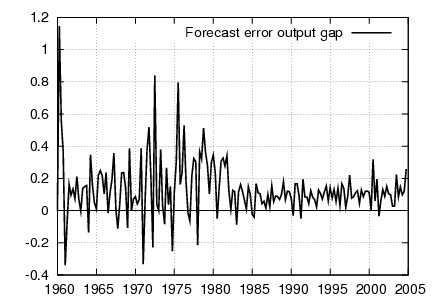
\includegraphics[scale=0.23]{plots2/diff_Forecast_error_output_gap.png} & 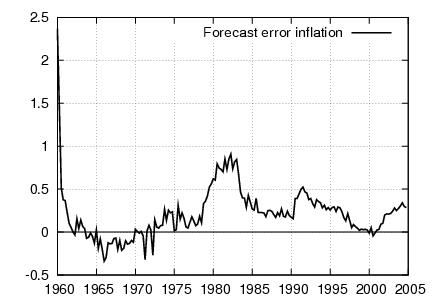
\includegraphics[scale=0.23]{plots2/diff_Forecast_error_inflation.png} & 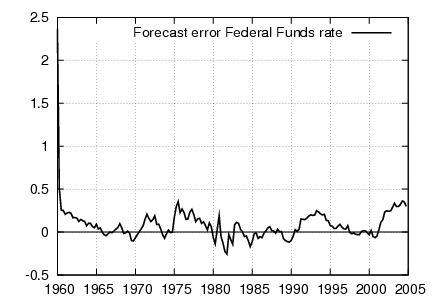
\includegraphics[scale=0.23]{plots2/diff_Forecast_error_Federal_Funds_rate.png} \\ \\
  \multicolumn{3}{c}{\textbf{Correlation of Forecast Errors}}  \\
  \small{Output gap} & \small{Inflation} & \small{Interest Rate} \\
  0.9858 & 0.9707 & 0.9833 \\
  \end{tabular}
  \end{center}
}

\frame
{
  \ft{Forecast Errors:\newline RE and Learning with RE initial conditions}
  \bi
  \item Forecast errors essentially the same.
  \item Forecast errors for all variables are largest in 1970s.
    \bi
    \item Neither model explains monetary policy in 1979-1982 period.
    \item Neither model can explain changes in volatility.
    \item Learning model actually makes slightly larger forecast errors.
    \ei
  \ei
}

\frame
{
  \ft{Smoothed Shocks\newline RE and Learning with RE initial conditions}
  \begin{center}
  \vspace*{-0.1in}\hspace*{-0.24in}\begin{tabular}{ccc}
  \multicolumn{3}{c}{\textbf{Rational Expectations}}  \\
  \small{Natural Rate Shock} & \small{Cost Push Shock} & \small{Policy Shock} \\
  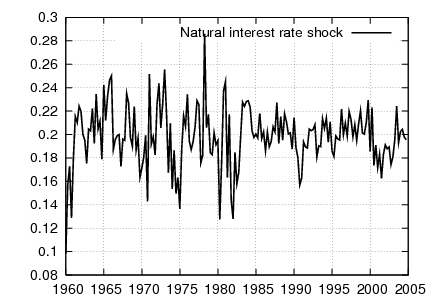
\includegraphics[scale=0.23]{plots2/re_natint.png} & 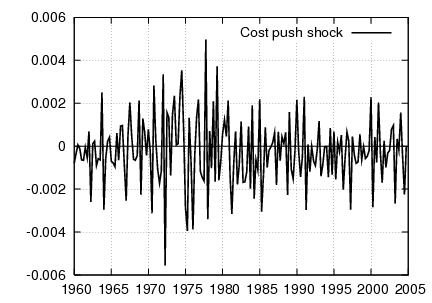
\includegraphics[scale=0.23]{plots2/re_costpush.png} & 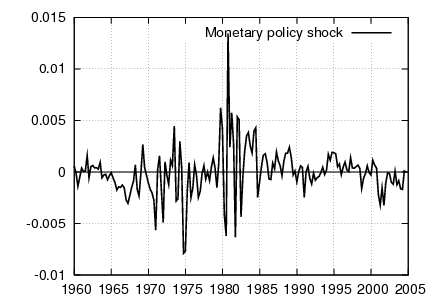
\includegraphics[scale=0.23]{plots2/re_mpshock.png} \\ \\
  \multicolumn{3}{c}{\textbf{Learning  (RE initial conditions)}}  \\
  \small{Natural Rate Shock} & \small{Cost Push Shock} & \small{Policy Shock} \\
  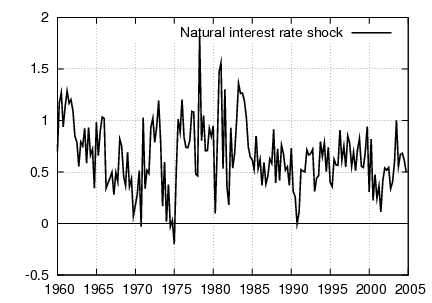
\includegraphics[scale=0.23]{plots2/initre_natint.png} & 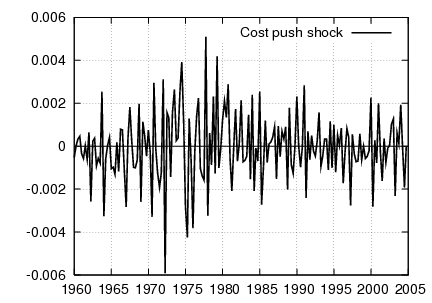
\includegraphics[scale=0.23]{plots2/initre_costpush.png} & 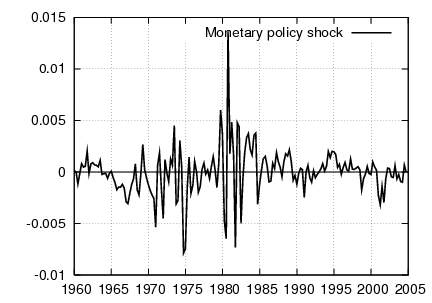
\includegraphics[scale=0.23]{plots2/initre_mpshock.png} \\ \\
  \end{tabular}
  \end{center}
}

\frame
{
  \ft{Smoothed Shocks\newline RE and Learning with RE initial conditions}
  \begin{center}
  \vspace*{-0.1in}\hspace*{-0.24in}\begin{tabular}{ccc}
  \multicolumn{3}{c}{\textbf{Difference in Smoothed Shocks}}  \\
  \small{Natural Rate Shock} & \small{Cost Push Shock} & \small{Policy Shock} \\
  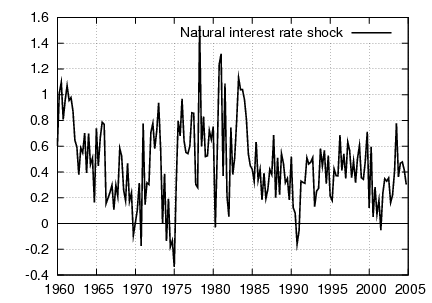
\includegraphics[scale=0.23]{plots2/diff_natint.png} & 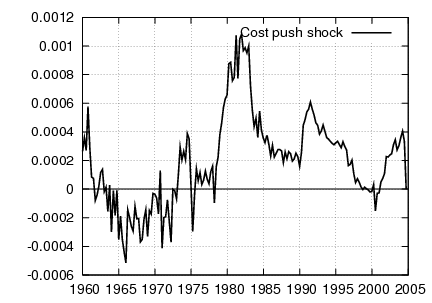
\includegraphics[scale=0.23]{plots2/diff_costpush.png} & 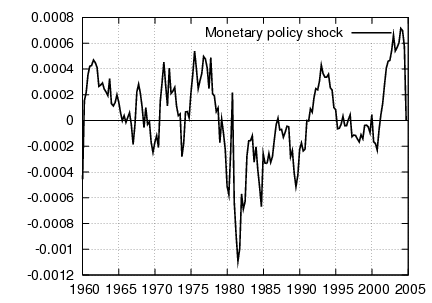
\includegraphics[scale=0.23]{plots2/diff_mpshock.png} \\ \\
  \multicolumn{3}{c}{\textbf{Correlation of Smoothed Shocks}}  \\
  \small{Natural Rate Shock} & \small{Cost Push Shock} & \small{Policy Shock} \\
  0.7150 & 0.9799 & 0.9907 \\
  \end{tabular}
  \end{center}
}

\frame
{
  \ft{Learning (RE initial conditions):\newline Evolution of Coefficients}
  \vspace*{-0.05in}\hspace*{-0.38in}\begin{tabular}{|cccc|} \hline
  \small{\textbf{Output:} Intercept} & \small{Output} & \small{Inflation} & \small{Fed Funds Rate} \\ \hline
  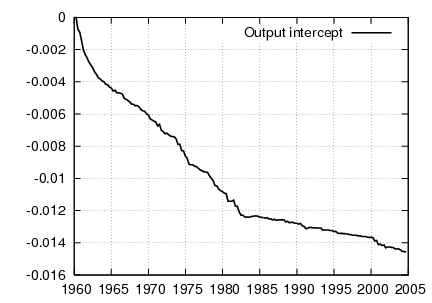
\includegraphics[scale=0.17]{plots2/initre_Output_intercept.png} &
  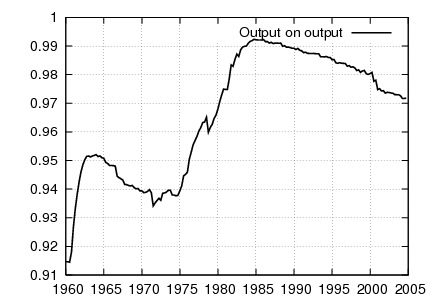
\includegraphics[scale=0.17]{plots2/initre_Output_on_output.png} &
  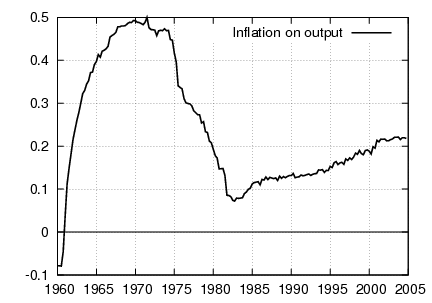
\includegraphics[scale=0.17]{plots2/initre_Inflation_on_output.png} & 
  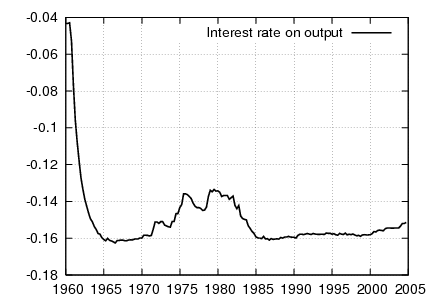
\includegraphics[scale=0.17]{plots2/initre_Interest_rate_on_output.png} \\ \hline
  \small{\textbf{Inflation:} Intercept} & \small{Output} & \small{Inflation} & \small{Fed Funds Rate} \\ \hline
  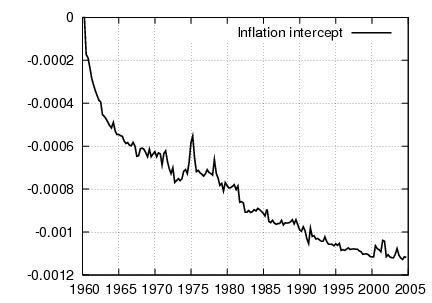
\includegraphics[scale=0.17]{plots2/initre_Inflation_intercept.png} &
  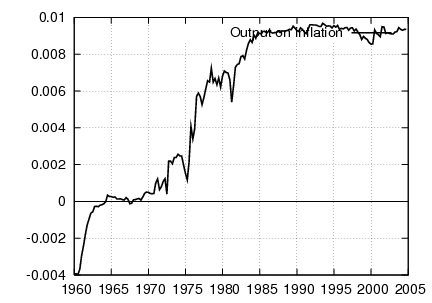
\includegraphics[scale=0.17]{plots2/initre_Output_on_inflation.png} &
  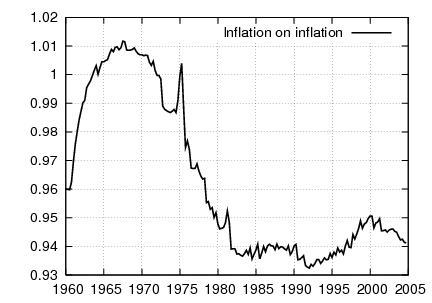
\includegraphics[scale=0.17]{plots2/initre_Inflation_on_inflation.png} & 
  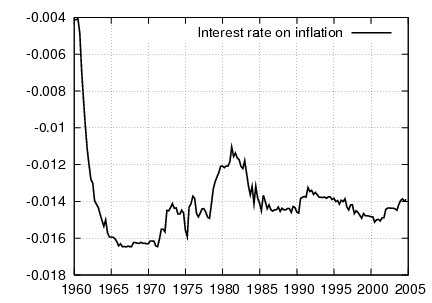
\includegraphics[scale=0.17]{plots2/initre_Interest_rate_on_inflation.png} \\ \hline
  \small{\textbf{Fed Funds:} Intercept} & \small{Output} & \small{Inflation} & \small{Fed Funds Rate} \\ \hline
  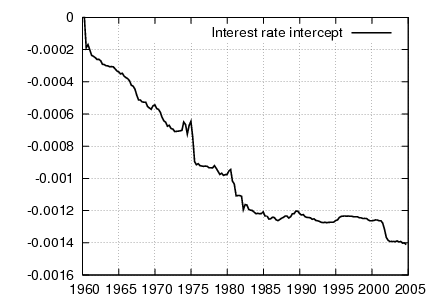
\includegraphics[scale=0.17]{plots2/initre_Interest_rate_intercept.png} &
  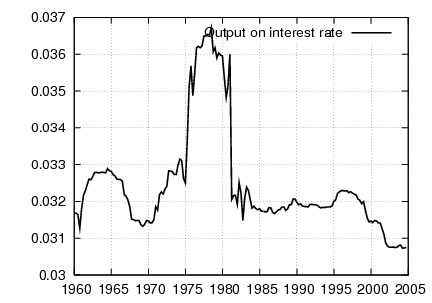
\includegraphics[scale=0.17]{plots2/initre_Output_on_interest_rate.png} &
  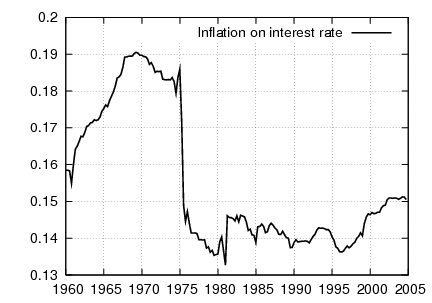
\includegraphics[scale=0.17]{plots2/initre_Inflation_on_interest_rate.png} & 
  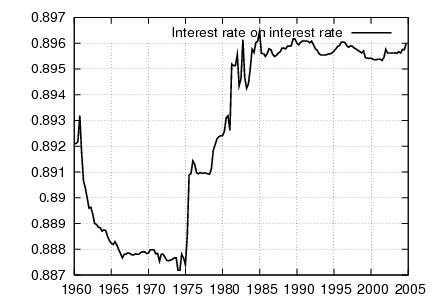
\includegraphics[scale=0.17]{plots2/initre_Interest_rate_on_interest_rate.png} \\ \hline
  \end{tabular}
}

\frame
{
  \ft{Learning (RE initial conditions):\newline Evolution of Coefficients}
  \bi
  \item Perceived persistence in output starts low, increases over the 1970s and early 1980s.
  \item Perceived impact of past inflation on output opposite sign of RE solution.
  \item Perceived persistence of inflation falls during 1970s.
  \item Perceived monetary policy during late 1970s:
    \bi
    \item Believed to respond more to output, less to inflation.
    \item Permanent increase in perceived interest rate persistence.
    \item Spike in the predictive power of interest rate.
    \ei
  \ei
}


\frame
{
\ft{Results Without Capital Accumulation:\newline Estimated Initial Conditions}
\begin{table}
\begin{scriptsize}
\begin{center}
\begin{tabular}{|l|c|r@{.}l|r@{.}l|} \hline
Description & Parameter & \multicolumn{2}{|c|}{Estimate} & \multicolumn{2}{|c|}{Std. dev.}  \\ \hline
Learning gain	&	$g$	&	0&0116	&	0&0072	\\
Habit formation	&	$\eta$	&	0&0436	&	0&0404	\\
Inverse elasticity sub.	&	$\sigma$	&	2&4018	&	2&8262	\\
Phillips curve slope	&	$\kappa$	&	0&0001	&	0&0003	\\
Price indexation	&	$\gamma$	&	0&9940	&	1&1123	\\
Interest rate smoothing	&	$\rho_r$	&	0&8940	&	0&0279	\\
Policy feedback on output	&	$\psi_y$	&	0&2973	&	0&1329	\\
Policy feedback on inflation	&	$\psi_{\pi}$	&	1&0576	&	0&1989	\\
Persistence nat. int. rate	&	$\rho_n$	&	0&9987	&	1&00E-8	\\
Persistence cost push	&	$\rho_u$	&	0&0002	&	0&0823	\\
Std. dev. nat. int. rate	&	$s_n$	&	0&0007	&	0&0080	\\
Std. dev. cost push	&	$s_u$	&	1&5E-05	&	6&06E-06	\\
Std. dev. policy shock	&	$s_r$	&	5&4E-06	&	4&6E-07	\\
Steady state inflation	&	$\pi^*$	&	1&6478	&	0&8418	\\ \hline
\end{tabular}
\end{center}
\end{scriptsize}
\end{table}
}

\frame
{
  \ft{Results Without Capital Accumulation:\newline Estimated Initial Conditions}
  \bi
  \item Not shown: estimates of initial conditions.  
    \bi
    \item Many estimates have large standard deviations.
    \ei
  \item Learning gain statistically significantly different from zero.
  \item Degree of habit formation is close to zero.
  \item Point estimate of price indexation still high, but insignificant.
  \item Point estimate of steady state inflation is low.
  \ei
}

\frame
{
  \ft{Forecast Errors:\newline RE and Learning with Estimated Initial Conditions}
  \begin{center}
  \vspace*{-0.1in}\hspace*{-0.24in}\begin{tabular}{ccc}
  \multicolumn{3}{c}{\textbf{Rational Expectations}}  \\
  \small{Output gap} & \small{Inflation} & \small{Interest Rate} \\
  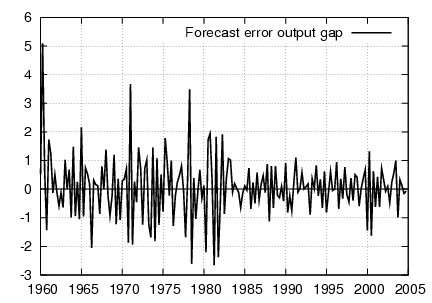
\includegraphics[scale=0.23]{plots2/re_Forecast_error_output_gap.png} & 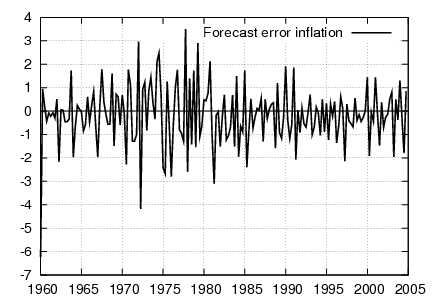
\includegraphics[scale=0.23]{plots2/re_Forecast_error_inflation.png} & 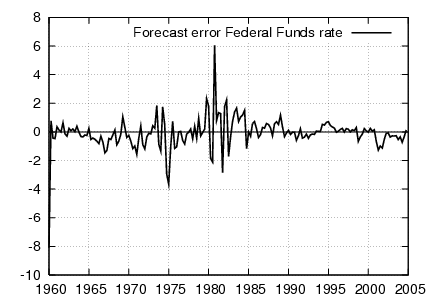
\includegraphics[scale=0.23]{plots2/re_Forecast_error_Federal_Funds_rate.png} \\ \\
  \multicolumn{3}{c}{\textbf{Learning (Estimated initial conditions)}}  \\
  \small{Output gap} & \small{Inflation} & \small{Interest Rate} \\
  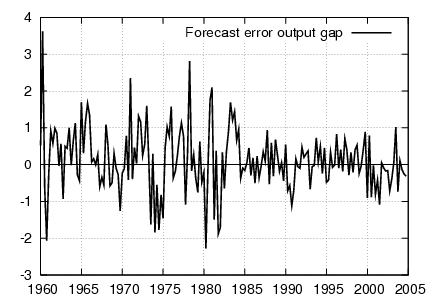
\includegraphics[scale=0.23]{plots2/initest_Forecast_error_output_gap.png} & 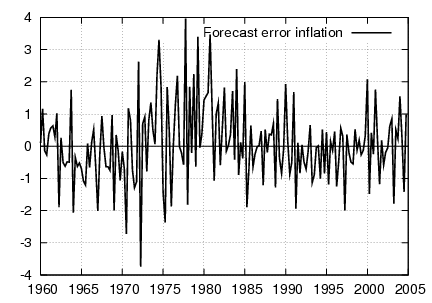
\includegraphics[scale=0.23]{plots2/initest_Forecast_error_inflation.png} & 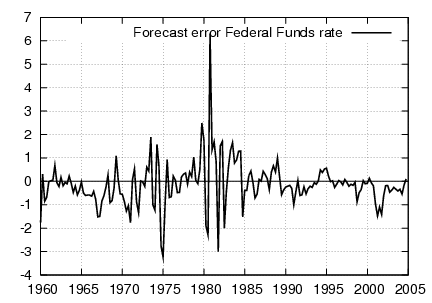
\includegraphics[scale=0.23]{plots2/initest_Forecast_error_Federal_Funds_rate.png} \\ \\
  \end{tabular}
  \end{center}
}

\frame
{
  \ft{Forecast Errors:\newline RE and Learning with Estimated Initial Conditions}
  \begin{center}
  \vspace*{-0.1in}\hspace*{-0.24in}\begin{tabular}{ccc}
  \multicolumn{3}{c}{\textbf{Differences in Forecast Errors}}  \\
  \small{Output gap} & \small{Inflation} & \small{Interest Rate} \\
  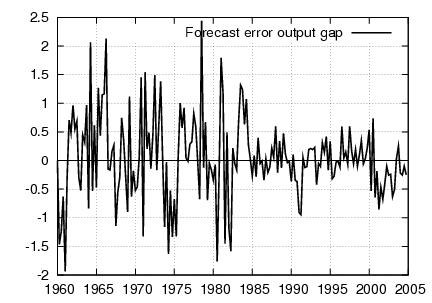
\includegraphics[scale=0.23]{plots2/diff_lnest_Forecast_error_output_gap.png} & 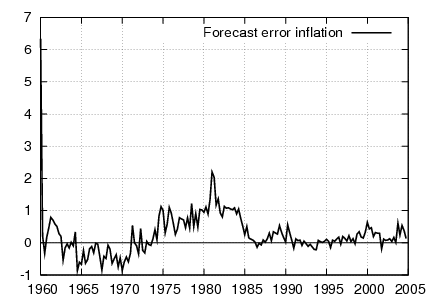
\includegraphics[scale=0.23]{plots2/diff_lnest_Forecast_error_inflation.png} & 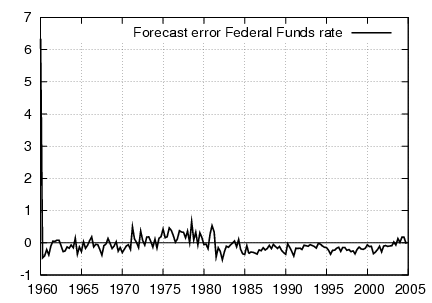
\includegraphics[scale=0.23]{plots2/diff_lnest_Forecast_error_Federal_Funds_rate.png} \\ \\
  \multicolumn{3}{c}{\textbf{Correlation of Forecast Errors}}  \\
  \small{Output gap} & \small{Inflation} & \small{Interest Rate} \\
  0.7333 & 0.8472 & 0.8861 \\
  \end{tabular}
  \end{center}
}

\frame
{
  \ft{Smoothed Shocks\newline RE and Learning with Estimated Initial Conditions}
  \begin{center}
  \vspace*{-0.1in}\hspace*{-0.24in}\begin{tabular}{ccc}
  \multicolumn{3}{c}{\textbf{Rational Expectations}}  \\
  \small{Natural Rate Shock} & \small{Cost Push Shock} & \small{Policy Shock} \\
  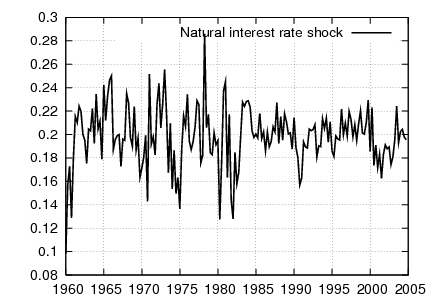
\includegraphics[scale=0.23]{plots2/re_natint.png} & 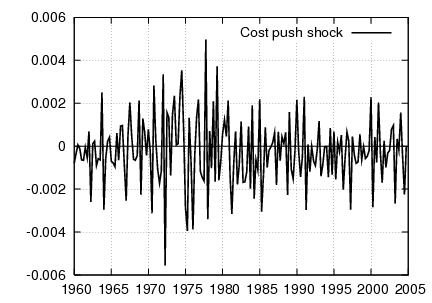
\includegraphics[scale=0.23]{plots2/re_costpush.png} & 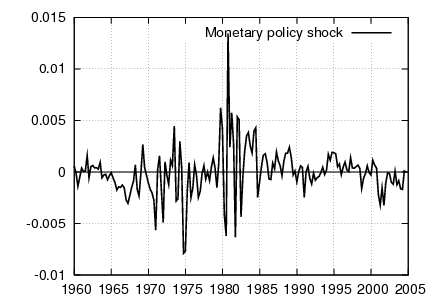
\includegraphics[scale=0.23]{plots2/re_mpshock.png} \\ \\
  \multicolumn{3}{c}{\textbf{Learning  (Estimated initial conditions)}}  \\
  \small{Natural Rate Shock} & \small{Cost Push Shock} & \small{Policy Shock} \\
  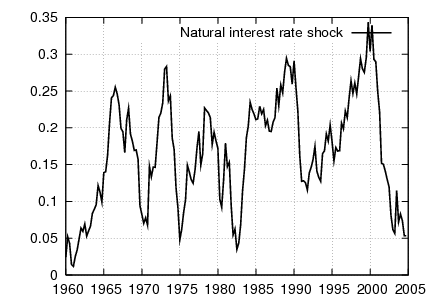
\includegraphics[scale=0.23]{plots2/initest_natint.png} & 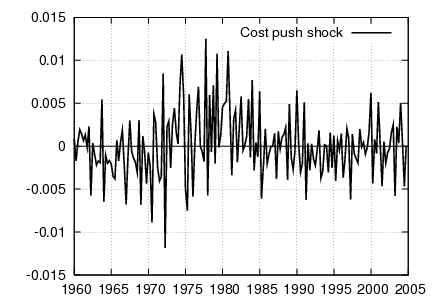
\includegraphics[scale=0.23]{plots2/initest_costpush.png} & 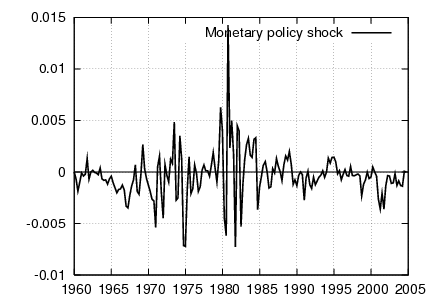
\includegraphics[scale=0.23]{plots2/initest_mpshock.png} \\ \\
  \end{tabular}
  \end{center}
}

\frame
{
  \ft{Smoothed Shocks\newline RE and Learning with Estimated Initial Conditions}
  \begin{center}
  \vspace*{-0.1in}\hspace*{-0.24in}\begin{tabular}{ccc}
  \multicolumn{3}{c}{\textbf{Difference in Smoothed Shocks}}  \\
  \small{Natural Rate Shock} & \small{Cost Push Shock} & \small{Policy Shock} \\
  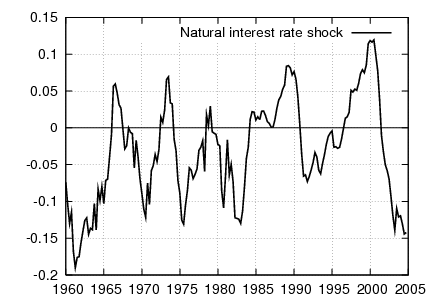
\includegraphics[scale=0.23]{plots2/diff_lnest_natint.png} & 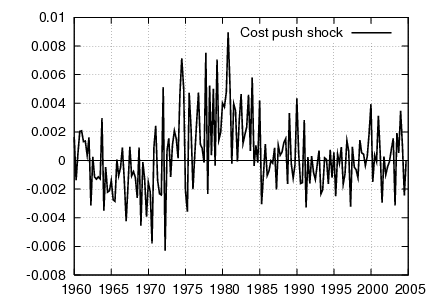
\includegraphics[scale=0.23]{plots2/diff_lnest_costpush.png} & 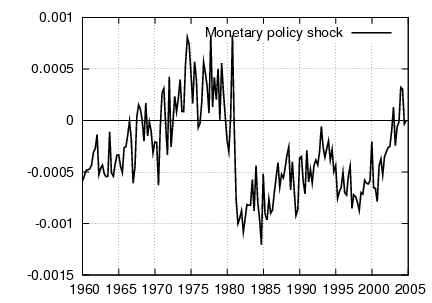
\includegraphics[scale=0.23]{plots2/diff_lnest_mpshock.png} \\ \\
  \multicolumn{3}{c}{\textbf{Correlation of Smoothed Shocks}}  \\
  \small{Natural Rate Shock} & \small{Cost Push Shock} & \small{Policy Shock} \\
  0.7150 & 0.9799 & 0.9907 \\
  \end{tabular}
  \end{center}
}

\frame
{
  \ft{Estimated Initial Conditions:\newline Evolution of Coefficients}
  \vspace*{-0.05in}\hspace*{-0.38in}\begin{tabular}{|cccc|} \hline
  \small{\textbf{Output:} Intercept} & \small{Output} & \small{Inflation} & \small{Fed Funds Rate} \\ \hline
  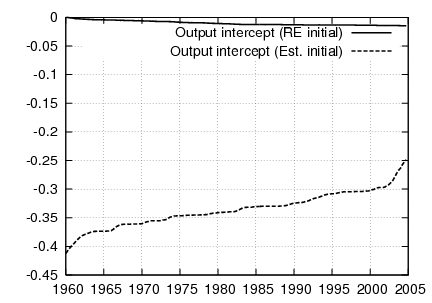
\includegraphics[scale=0.17]{plots2/initest_Output_intercept.png} &
  \includegraphics[scale=0.17]{plots2/initest_Output_on_output.png} &
  \includegraphics[scale=0.17]{plots2/initest_Inflation_on_output.png} & 
  \includegraphics[scale=0.17]{plots2/initest_Interest_rate_on_output.png} \\ \hline
  \small{\textbf{Inflation:} Intercept} & \small{Output} & \small{Inflation} & \small{Fed Funds Rate} \\ \hline
  \includegraphics[scale=0.17]{plots2/initest_Inflation_intercept.png} &
  \includegraphics[scale=0.17]{plots2/initest_Output_on_inflation.png} &
  \includegraphics[scale=0.17]{plots2/initest_Inflation_on_inflation.png} & 
  \includegraphics[scale=0.17]{plots2/initest_Interest_rate_on_inflation.png} \\ \hline
  \small{\textbf{Fed Funds:} Intercept} & \small{Output} & \small{Inflation} & \small{Fed Funds Rate} \\ \hline
  \includegraphics[scale=0.17]{plots2/initest_Interest_rate_intercept.png} &
  \includegraphics[scale=0.17]{plots2/initest_Output_on_interest_rate.png} &
  \includegraphics[scale=0.17]{plots2/initest_Inflation_on_interest_rate.png} & 
  \includegraphics[scale=0.17]{plots2/initest_Interest_rate_on_interest_rate.png} \\ \hline
  \end{tabular}
}


\frame
{
  \ft{Some More Model Comparisons}
  \hspace{-0.1in}\begin{tabular}{|c|ccc|} \hline
   & RE & Learning (RE init.) & Learning (Est. init.) \\ \hline
  MSE Output & 1.0920 & 1.1041 & 0.7303 \\
  MSE Inflation & 1.6613 & 1.5781 & 1.4175 \\
  MSE Fed Funds & 1.2594 & 1.0879 & 0.9435 \\ 
  Log-likelihood & -303.8 & -291.9 & -241.6 \\ \hline
  \end{tabular}
}

\frame
{
\ft{Results With Capital Accumulation:\newline RE Solution for Initial Conditions}
\vspace*{-0.08in}
\hspace*{-0.12in}
\begin{scriptsize}
\hspace{-0.2in}
\begin{tabular}{|l|c|r@{.}l|r@{.}l|r@{.}l|r@{.}l|} \hline
Description & Parameter & \multicolumn{2}{|c|}{RE} & \multicolumn{2}{|c|}{Std. dev.} & \multicolumn{2}{|c|}{Learning} & \multicolumn{2}{|c|}{Std. dev.}  \\ \hline
Learning gain	&	$g$	&	&	&	&	&	3&51E-6	&	7&01E-6	\\
Habit formation	&	$\eta$	&	0&0855	&	0&0846	&	0&1078	&	0&0805	\\
Inverse elasticity sub.	&	$\sigma$	&	16&5056	&	13&8189	&	16&8358	&	14&5459	\\
Capital / output ratio	&	$k_y$	&	4&4799	&	0&2129	&	4&5061	&	0&2129	\\
Consumption / output ratio	&	$c_y$	&	0&7141	&	0&0547	&	0&7234	&	0&0516	\\
Inverse elasticity labor	&	$\mu$	&	1&53E-5	&	0&3944	&	1&00E-5	&	0&4396	\\
Capital adjustment cost	&	$\phi$	&	27&9001	&	5&4801	&	27&4460	&	5&9845	\\
Phillips curve slope	&	$\kappa$	&	0&0116	&	0&0034	&	0&0119	&	0&0037	\\
Price indexation	&	$\gamma$	&	0&9999	&	0&0000	&	0&9999	&	0&0000	\\
Interest rate smoothing	&	$\rho_r$	&	0&8147	&	0&0196	&	0&8103	&	0&0203	\\
Policy feedback on output	&	$\psi_y$	&	0&0326	&	0&0116	&	0&0356	&	0&0122	\\
Policy feedback on inflation	&	$\psi_{\pi}$	&	1&5401	&	0&1504	&	1&4735	&	0&1405	\\
Persistence in tech. shock	&	$\rho_z$	&	1&40E-5	&	0&0888	&	1&00E-5	&	0&0902	\\
Persistence in pref. shock	&	$\rho_{\xi}$	&	0&9793	&	0&0176	&	0&9800	&	0&0167	\\
Persistence in inv. shock	&	$\rho_{\mu}$	&	0&9295	&	0&0235	&	0&9282	&	0&0253	\\
Persistence in AD shock	&	$\rho_g$	&	0&9989	&	0&0042	&	0&9993	&	0&0035	\\
Std. dev. tech. shock	&	$s_z$	&	0&2399	&	0&1262	&	0&2326	&	0&1325	\\
Std. dev. inv. shock	&	$s_{\mu}$	&	0&1996	&	0&1219	&	0&1900	&	0&1251	\\
Std. dev. pref. shock	&	$s_{\xi}$	&	0&1722	&	0&1447	&	0&1857	&	0&1626	\\
Std. dev. policy shock	&	$s_r$	&	0&0025	&	0&0001	&	0&0024	&	0&0001	\\
Std. dev. AD shock	&	$s_g$	&	0&0222	&	0&0091	&	0&0238	&	0&0098	\\
Steady state inflation	&	$\pi^{*}$	&	8&6918	&	2&3997	&	10&3678	&	3&0793	\\
Steady state output	&	$y^{*}$	&	1&2521	&	0&1033	&	1&2355	&	0&0984	\\ \hline
\end{tabular}
\end{scriptsize}
}

\frame
{
\ft{Results With Capital Accumulation:\newline Estimated Initial Conditions}
\begin{scriptsize}
\vspace*{-0.15in}
\begin{center}
\begin{tabular}{|l|c|r@{.}l|r@{.}l|} \hline
Description & Parameter & \multicolumn{2}{|c|}{Estimate} & \multicolumn{2}{|c|}{Std. dev.}  \\ \hline
Learning gain	&	$g$	&	0&0288	&	0&0077	\\
Habit formation	&	$\eta$	&	0&0772	&	0&1031	\\
Inverse elasticity sub.	&	$\sigma$	&	16&6941	&	14&4002	\\
Capital / output ratio	&	$k_y$	&	4&5086	&	1&5187	\\
Consumption / output ratio	&	$c_y$	&	0&7213	&	0&0842	\\
Inverse elasticity labor	&	$\mu$	&	0&0132	&	1&3992	\\
Capital adjustment cost	&	$\phi$	&	28&1764	&	38&5551	\\
Phillips curve slope	&	$\kappa$	&	0&0120	&	0&0154	\\
Price indexation	&	$\gamma$	&	0&9999	&	0&0000	\\
Interest rate smoothing	&	$\rho_r$	&	0&8776	&	0&0351	\\
Policy feedback on output	&	$\psi_y$	&	0&0374	&	0&0661	\\
Policy feedback on inflation	&	$\psi_{\pi}$	&	1&5654	&	0&4185	\\
Persistence in tech. shock	&	$\rho_z$	&	0&0000	&	0&0124	\\
Persistence in pref. shock	&	$\rho_{\xi}$	&	0&9611	&	0&0234	\\
Persistence in inv. shock	&	$\rho_{\mu}$	&	0&9364	&	0&0405	\\
Persistence in AD shock	&	$\rho_g$	&	0&9999	&	0&0001	\\
Std. dev. tech. shock	&	$s_z$	&	0&2569	&	0&5566	\\
Std. dev. inv. shock	&	$s_{\mu}$	&	0&1830	&	0&1692	\\
Std. dev. pref. shock	&	$s_{\xi}$	&	0&1707	&	0&1461	\\
Std. dev. policy shock	&	$s_r$	&	0&0024	&	0&0001	\\
Std. dev. AD shock	&	$s_g$	&	0&0255	&	0&0154	\\
Steady state inflation	&	$\pi^{*}$	&	9&5185	&	6&1255	\\
Steady state output	&	$y^{*}$	&	1&2396	&	0&1424	\\ \hline
\end{tabular}
\end{center}
\end{scriptsize}
}


\frame
{
  \ft{Results With Capital Accumulation}
  \bi
  \item With RE initial conditions:
    \bi
    \item Learning gain essentially zero.
    \item All parameter estimates are very similar.
    \item Habit formation close to zero under \textit{both} RE and Learning.
    \item Inflation indexation very close to one.
    \ei
  \item With Estimated initial conditions.
    \bi
    \item Point estimates similar as with RE.
    \item Not shown: standard deviations for some initial conditions huge.
    \item Learning gain greater than zero.
    \item Inflation indexation remains significant and close to one.
    \item Standard deviations of some structural parameters increased:
      \bi 
      \item Capital adjustment cost.
      \item Policy feedback on inflation.
      \item Steady state inflation.
      \ei
    \ei
  \ei
}

\frame
{
  \ft{Forecast Errors:\newline RE and Learning with RE Initial Conditions}
  \begin{center}
  \vspace*{-0.1in}\hspace*{-0.24in}\begin{tabular}{ccc}
  \multicolumn{3}{c}{\textbf{Rational Expectations}}  \\
  \small{Output} & \small{Consumption} & \small{Investment} \\
  \includegraphics[scale=0.23]{plots2/cap_re_Forecast_error_output.png} & \includegraphics[scale=0.23]{plots2/cap_re_Forecast_error_consumption.png} & \includegraphics[scale=0.23]{plots2/cap_re_Forecast_error_investment.png} \\ \\
  \small{Inflation} & \small{Interest Rate} & \\
  \includegraphics[scale=0.23]{plots2/cap_re_Forecast_error_inflation.png} & \includegraphics[scale=0.23]{plots2/cap_re_Forecast_error_Federal_Funds_rate.png} & \\ \\
  \end{tabular}
  \end{center}
}

\frame
{
  \ft{Forecast Errors:\newline RE and Learning with RE Initial Conditions}
  \begin{center}
  \vspace*{-0.1in}\hspace*{-0.24in}\begin{tabular}{ccc}
  \multicolumn{3}{c}{\textbf{Learning (RE initial conditions)}}  \\
  \small{Output} & \small{Consumption} & \small{Investment} \\
  \includegraphics[scale=0.23]{plots2/cap_initre_Forecast_error_output.png} & \includegraphics[scale=0.23]{plots2/cap_initre_Forecast_error_consumption.png} & \includegraphics[scale=0.23]{plots2/cap_initre_Forecast_error_investment.png} \\ \\
  \small{Inflation} & \small{Interest Rate} & \\
  \includegraphics[scale=0.23]{plots2/cap_initre_Forecast_error_inflation.png} & \includegraphics[scale=0.23]{plots2/cap_initre_Forecast_error_Federal_Funds_rate.png} & \\ \\
  \end{tabular}
  \end{center}
}

\frame
{
  \ft{Forecast Errors:\newline RE and Learning with RE Initial Conditions}
  \begin{center}
  \vspace*{-0.2in}\hspace*{-0.24in}\begin{tabular}{ccc}
  \multicolumn{3}{c}{\textbf{Differences in Forecast Errors (Correlations)}}  \\
  \small{Output} & \small{Consumption} & \small{Investment} \\
  \includegraphics[scale=0.23]{plots2/cap_diff_Forecast_error_output.png} & \includegraphics[scale=0.23]{plots2/cap_diff_Forecast_error_consumption.png} & \includegraphics[scale=0.23]{plots2/cap_diff_Forecast_error_investment.png} \\
  (0.9966) & (0.9997) & (0.9982) \\ 
  \small{Inflation} & \small{Interest Rate} & \\
  \includegraphics[scale=0.23]{plots2/cap_diff_Forecast_error_inflation.png} & \includegraphics[scale=0.23]{plots2/cap_diff_Forecast_error_Federal_Funds_rate.png} & \\
  (0.9956) & (0.9968) & \\ \\

  \end{tabular}
  \end{center}
}

\frame
{
  \ft{Forecast Errors:\newline RE and Learning with Estimated Initial Conditions}
  \begin{center}
  \vspace*{-0.1in}\hspace*{-0.24in}\begin{tabular}{ccc}
  \multicolumn{3}{c}{\textbf{Learning (Estimated initial conditions)}}  \\
  \small{Output} & \small{Consumption} & \small{Investment} \\
  \includegraphics[scale=0.23]{plots2/cap_initest_Forecast_error_output.png} & \includegraphics[scale=0.23]{plots2/cap_initest_Forecast_error_consumption.png} & \includegraphics[scale=0.23]{plots2/cap_initest_Forecast_error_investment.png} \\ \\
  \small{Inflation} & \small{Interest Rate} & \\
  \includegraphics[scale=0.23]{plots2/cap_initest_Forecast_error_inflation.png} & \includegraphics[scale=0.23]{plots2/cap_initest_Forecast_error_Federal_Funds_rate.png} & \\ \\
  \end{tabular}
  \end{center}
}

\frame
{
  \ft{Forecast Errors:\newline RE and Learning with Estimated Initial Conditions}
  \begin{center}
  \vspace*{-0.2in}\hspace*{-0.24in}\begin{tabular}{ccc}
  \multicolumn{3}{c}{\textbf{Differences in Forecast Errors (Correlations)}}  \\
  \small{Output} & \small{Consumption} & \small{Investment} \\
  \includegraphics[scale=0.23]{plots2/cap_diff_lnest_Forecast_error_output.png} & \includegraphics[scale=0.23]{plots2/cap_diff_lnest_Forecast_error_consumption.png} & \includegraphics[scale=0.23]{plots2/cap_diff_lnest_Forecast_error_investment.png} \\
  (0.9213) & (0.9906) & (0.7294) \\ 
  \small{Inflation} & \small{Interest Rate} & \\
  \includegraphics[scale=0.23]{plots2/cap_diff_lnest_Forecast_error_inflation.png} & \includegraphics[scale=0.23]{plots2/cap_diff_lnest_Forecast_error_Federal_Funds_rate.png} & \\
  (0.9527) & (0.9847) & \\ \\
  \end{tabular}
  \end{center}
}

\frame
{
  \ft{Forecast Errors for Endogenous Capital model}
  \bi
  \item Forecast errors for inflation and federal funds rate are clustered in 1970s.
  \item Volatility of forecast errors is not clustered for consumption and investment.
  \item Learning model with estimated initial conditions:
    \bi
    \item Out performs the RE model for predicting inflation during 1970s.
    \item Under performs the RE model for predicting output during 1980s.
    \ei
  \item Even with estimated initial conditions: models have similar performance.
  \ei
}


\frame
{
  \ft{Smoothed Shocks:\newline RE and Learning with RE Initial Conditions}
  \begin{center}
  \vspace*{-0.1in}\hspace*{-0.24in}\begin{tabular}{ccc}
  \multicolumn{3}{c}{\textbf{Rational Expectations}}  \\
  \small{Technology shock} & \small{Investment shock} & \small{Monetary policy shock} \\
  \includegraphics[scale=0.23]{plots2/cap_re_techsh.png} & \includegraphics[scale=0.23]{plots2/cap_re_invsh.png} & \includegraphics[scale=0.23]{plots2/cap_re_mpshock.png} \\ \\
  \small{Preference shock} & \small{Aggregate demand shock} & \\
  \includegraphics[scale=0.23]{plots2/cap_re_prefsh.png} & \includegraphics[scale=0.23]{plots2/cap_re_ADsh.png} & \\ \\
  \end{tabular}
  \end{center}
}

\frame
{
  \ft{Smoothed Shocks:\newline RE and Learning with RE Initial Conditions}
  \begin{center}
  \vspace*{-0.1in}\hspace*{-0.24in}\begin{tabular}{ccc}
  \multicolumn{3}{c}{\textbf{Learning (RE initial conditions)}}  \\
  \small{Technology shock} & \small{Investment shock} & \small{Monetary policy shock} \\
  \includegraphics[scale=0.23]{plots2/cap_initre_techsh.png} & \includegraphics[scale=0.23]{plots2/cap_initre_invsh.png} & \includegraphics[scale=0.23]{plots2/cap_initre_mpshock.png} \\ \\
  \small{Preference shock} & \small{Aggregate demand shock} & \\
  \includegraphics[scale=0.23]{plots2/cap_initre_prefsh.png} & \includegraphics[scale=0.23]{plots2/cap_initre_ADsh.png} & \\ \\
  \end{tabular}
  \end{center}
}

\frame
{
  \ft{Smoothed Shocks:\newline RE and Learning with RE Initial Conditions}
  \begin{center}
  \vspace*{-0.2in}\hspace*{-0.24in}\begin{tabular}{ccc}
  \multicolumn{3}{c}{\textbf{Differences in smoothed shocks (Correlations)}}  \\
  \small{Technology shock} & \small{Investment shock} & \small{Monetary policy shock} \\
  \includegraphics[scale=0.23]{plots2/cap_diff_techsh.png} & \includegraphics[scale=0.23]{plots2/cap_diff_invsh.png} & \includegraphics[scale=0.23]{plots2/cap_diff_mpshock.png} \\ 
  (0.9996) & (0.9998) & (0.9997) \\ 
  \small{Preference shock} & \small{Aggregate demand shock} & \\
  \includegraphics[scale=0.23]{plots2/cap_diff_prefsh.png} & \includegraphics[scale=0.23]{plots2/cap_diff_ADsh.png} & \\
  (0.9998) & (0.9999) &  \\ 

  \end{tabular}
  \end{center}
}


\frame
{
  \ft{Smoothed Shocks:\newline RE and Learning with Estimated Initial Conditions}
  \begin{center}
  \vspace*{-0.1in}\hspace*{-0.24in}\begin{tabular}{ccc}
  \multicolumn{3}{c}{\textbf{Learning (Estimated initial conditions)}}  \\
  \small{Technology shock} & \small{Investment shock} & \small{Monetary policy shock} \\
  \includegraphics[scale=0.23]{plots2/cap_initest_techsh.png} & \includegraphics[scale=0.23]{plots2/cap_initest_invsh.png} & \includegraphics[scale=0.23]{plots2/cap_initest_mpshock.png} \\ \\
  \small{Preference shock} & \small{Aggregate demand shock} & \\
  \includegraphics[scale=0.23]{plots2/cap_initest_prefsh.png} & \includegraphics[scale=0.23]{plots2/cap_initre_ADsh.png} & \\ \\
  \end{tabular}
  \end{center}
}

\frame
{
  \ft{Smoothed Shocks:\newline RE and Learning with Estimated Initial Conditions}
  \begin{center}
  \vspace*{-0.2in}\hspace*{-0.24in}\begin{tabular}{ccc}
  \multicolumn{3}{c}{\textbf{Differences in smoothed shocks (Correlations)}}  \\
  \small{Technology shock} & \small{Investment shock} & \small{Monetary policy shock} \\
  \includegraphics[scale=0.23]{plots2/cap_diff_lnest_techsh.png} & \includegraphics[scale=0.23]{plots2/cap_diff_lnest_invsh.png} & \includegraphics[scale=0.23]{plots2/cap_diff_lnest_mpshock.png} \\ 
  (-0.9528) & (0.5308) & (0.9794) \\ 
  \small{Preference shock} & \small{Aggregate demand shock} & \\
  \includegraphics[scale=0.23]{plots2/cap_diff_lnest_prefsh.png} & \includegraphics[scale=0.23]{plots2/cap_diff_lnest_ADsh.png} & \\
  (0.9760) & (0.9999) &  \\ 

  \end{tabular}
  \end{center}
}

\frame
{
  \ft{Comparison of Coefficients}
  \vspace*{-0.02in}\hspace*{-0.38in}\begin{tabular}{|cccc|} \hline
  \small{\textbf{Output:} Output} & \small{Inflation} & \small{Fed Funds Rate} & \small{Capital} \\ \hline
  \includegraphics[scale=0.17]{plots2/cap_initest_Output_on_output.png} &
  \includegraphics[scale=0.17]{plots2/cap_initest_Inflation_on_output.png} &
  \includegraphics[scale=0.17]{plots2/cap_initest_Interest_rate_on_output.png} & 
  \includegraphics[scale=0.17]{plots2/cap_initest_Capital_on_output.png} \\ \hline
  \small{\textbf{Inflation:} Output} & \small{Inflation} & \small{Fed Funds Rate} & \small{Capital} \\ \hline
  \includegraphics[scale=0.17]{plots2/cap_initest_Output_on_inflation.png} &
  \includegraphics[scale=0.17]{plots2/cap_initest_Inflation_on_inflation.png} &
  \includegraphics[scale=0.17]{plots2/cap_initest_Interest_rate_on_inflation.png} & 
  \includegraphics[scale=0.17]{plots2/cap_initest_Capital_on_inflation.png} \\ \hline
  \small{\textbf{Capital:} Output} & \small{Inflation} & \small{Fed Funds Rate} & \small{Capital} \\ \hline
  \includegraphics[scale=0.17]{plots2/cap_initest_Output_on_capital.png} &
  \includegraphics[scale=0.17]{plots2/cap_initest_Inflation_on_capital.png} &
  \includegraphics[scale=0.17]{plots2/cap_initest_Interest_rate_on_capital.png} & 
  \includegraphics[scale=0.17]{plots2/cap_initest_Capital_on_capital.png} \\ \hline
  \end{tabular}
}

\frame
{
  \ft{Some More Model Comparisons}
  \hspace{-0.48in}\begin{tabular}{|c|ccc|} \hline
   & RE & Learning (RE init.) & Learning (Est. init.) \\ \hline
  MSE Output & 23558.2 & 24868.6 & 24652.0 \\
  MSE Consumption & 7129.3 & 7105.1 & 6883.4 \\
  MSE Investment & 7118.3 & 6930.3 & 7656.7 \\
  MSE Inflation & 1.6727 & 1.7508 & 1.3893 \\
  MSE Fed Funds & 1.4116 & 1.5910 & 1.4483 \\ 
  Log-likelihood & -3042.2 & -3041.6 & -241.6 \\ \hline
  \end{tabular}
}

\frame
{
  \ft{Conclusion}
  \bi
  \item Estimated a NK model without capital under RE and Learning.
    \bi
    \item RE initial conditions: fails to explain persistence, volatility clustering.
    \item Estimated initial conditions: some persistence explained, not volatility clustering.
    \ei
  \item Estimated a NK model with endogenous capital under RE and learning.
    \bi
    \item Using RE initial conditions: No difference, capital explained some persistence and volatility.
    \item Using Estimated Initial conditions: 
      \bi
      \item Can get very different paths of shocks and coefficients.
      \item Model fit not greatly improved.
      \item Still does not explain volatility clustering.
      \ei
    \ei
  \item Conclusion: Expectations framework with larger deviations from RE likely needed to explain data.
  \ei
}

\end{document}

